\documentclass[11pt,a4paper]{scrreprt}
\usepackage[utf8]{inputenc}
\usepackage[german]{babel}
\usepackage[T1]{fontenc}
\usepackage{amssymb}
\usepackage{graphicx}
\usepackage{enumitem}

%--- PDF Dokumenteninformation ---
\usepackage[
		pdftitle={Sanfilippo - Lernen mit Podcasts},
		pdfsubject={},
		pdfauthor={Martin Sanfilippo},
		pdfkeywords={},
		hidelinks
]{hyperref}

%--- Besondere Wort-Trennung ---
\hyphenation{De-zi-mal-tren-nung}

%--- Quellenverzeichnis ---
\bibliographystyle{apalike}

%--- Abkürzungsverzeichnis (nur genutzte anzeigen) ---
\usepackage[printonlyused]{acronym}

%--- schicke Kopf- und Fusszeile ---
\usepackage{fancyhdr}
\usepackage[left = 2.5cm,right = 2cm,top = 3cm,bottom = 3cm]{geometry}

\pagestyle{fancy}
\lhead{\slshape Martin Sanfilippo - 862013}
\chead{}
\rhead{\slshape Lernen mit Podcasts}

\lfoot{}
\cfoot{\thepage}
\rfoot{}

\renewcommand{\headrulewidth}{0.2pt}
\renewcommand{\footrulewidth}{0pt}

%--- Inhalt Titelblatt ---
\author{Martin Sanfilippo - 862013}
\title{Lernen mit Podcasts: Möglichkeiten und Grenzen}

\begin{document}

%--- Textbereich --- 

\begin{titlepage}
	\centering
	\begin{figure}[h]
	\begin{center}
	
\includegraphics[width=0.15\textwidth]{Feed-icon}\par\vspace{1cm}
	\setbox0=\vbox{ \caption{Mozilla Foundation under a MPL/GPL/LGPL tri-license.\cite{MozillaFoundation1995}}}
	\label{Podcastlogo}
	\end{center}
	\end{figure}
	{\slshape\LARGE Beuth Hochschule für Technik Berlin \par}
	\vspace{1cm}
	{\slshape\Large Einführung in die wissenschaftliche Projektarbeit\\(BHTB MIB 13 S18)\par}
	\vspace{4cm}
	{\huge\bfseries Lernen mit Podcasts: \\Möglichkeiten und Grenzen\par}
	\vspace{4cm}
	{\Large\slshape Martin Sanfilippo - 862013\\
	\small Studiensemester 4\\
	\small Fachsemester 4\par}
	\vfill
	betreut durch\par
	Professor Larysa Visengeriyeva

	\vfill

% Bottom of the page
	{\large \today\par}
\end{titlepage}


\chapter{Einleitung}
\thispagestyle{fancy}
\setcounter{page}{1} 
Bereits seit 2010 produziere ich selbst Audio-Podcasts, daher ist dieses Themenfeld für mich aus vielerlei Sicht interessant: Einerseits aus der Betrachtung als Producer, der eine möglichst große Verbreitung erreichen und begeisterte Zuhörer haben möchte, andererseits ist auch aus der Pespektive der Konsumenten das Thema ``Podcast`` sehr interessant. Denn mich betrifft, was auch für einen Großteil der Podcast-Producer gilt, wir sind vom Konsumenten zum Prosument geworden. \\ Der Begriff ``Prosument`` stammt vom englischen ``Prosumer`` und wird aus den Begriffen Producer, zu Deutsch Produzent, und Consumer, zu Deutsch Konsument, zusammengesetzt. In Rückbezug auf das Verständnis vom Futurologen Toffler aus dem Jahr 1980, erfasst die Zusammensetzung der Begrifflichkeiten den Sachverhalt treffend \cite{SusannaRasch2016}.\\ 
Befähigt durch die Demokratisierung und Individualisierung von Informationen und Inhalten erhebt sich der Konsument schließlich zu einem selbstbestimmten und gleichberechtigten Prosumenten, der Unternehmen und Institutionen auf Augenhöhe begegnet und seine Erwartungen und Präferenzen selbstsicher vertritt \cite[S. 1]{Michelis2014}. \\
Die Prosumenten streben nach Partizipation und so können sie, befähigt durch die kommunikationstechnologischen Entwicklungen, bei einem Thema ihrer Wahl mitgestalten und selbst eine Marke und Kultur entwickeln.\\ So streben Prosumenten nicht ausschließlich nach Individualisierung, sie wollen diese in Form einer Verbundenheit mit Gleichgesinnten ausleben und sich in entsprechenden sozialen Gruppen, sogenannten Communities, vernetzen \cite[S. 308] {Baumann2014}. \\
Durch die gefühlte Nähe der Konsumenten zum Sprecher des Podcasts entwickelt sich eine persönliche Ebene, die viele motiviert, es nicht nur bei einem bloßen Zuhören zu belassen, sondern sich einzubringen. Das Spektrum des Engagements reicht von ausgiebigem Feedback über finanzielle Unterstützung bis hin zum Wechsel vom Konsumenten zum Prosumenten. Dies stärkt die Community und motiviert die Producer durch die anhaltende Rückkoppelung. 

\chapter{Zusammenfassung}
\thispagestyle{fancy}
Seit 2004 hat sich der Podcast-Markt stark entwickelt, was am aktuellen Marktführer für Podcastverzeichnisse gesehen werden kann. Auf der WWDC\footnote{Die Apple Worldwide Developers Conference ist eine jährlich in Kalifornien veranstaltete Software-Entwickler-Konferenz.} 2018 zählte ``Apple iTunes`` bereits über 550.000 Podcasts und seit dem Start der Plattform über 50 Milliarden Downloads einzelner Episoden, davon allein im Jahr 2017 13,7 Milliarden Downloads. Dies deutet auf einen schnell wachsenden Markt hin \cite{Heater2018}.\\ 
Podcasts scheinen damit kein Nischenangebot mehr zu sein, sondern sind im Mainstream angekommen. Durch den geringen Aufwand und die niedrigen Produktionskosten kommen sie inzwischen mit einem breiten Spektrum beim Abonnenten an. Selbst Themen mit nur geringer Interessentenzahl werden bedient. Aber sogar bei den großen Abrufzahlen ist das zukünftige Potential noch umfangreich. Aus der aktuellen ARD/ZDF-Onlinestudie\footnote{http://www.ard-zdf-onlinestudie.de (zuletzt zugegriffen 18.06.2018) \cite{ARD/ZDF-Medienkommission2017}} von 2017 geht hervor, dass in Deutschland nur 3 \% der befragten regelmäßig Podcasts hören. Gesamtgesellschaftlich spielt der Podcast in Deutschland folglich noch keine tragende Rolle.\\In den USA hingegen ist der Podcast-Markt dem deutschen Markt einige Jahre voraus. Dort steigt der Anteil der Podcast-Nutzer ebenso stetig an, jedoch auf einem anderen Niveau. Von 2017 auf 2018 stieg der Anteil der US-amerikanischen Bevölkerung, die Podcasts nutzten, von 40 \% auf 44 \% an \cite{Statista2018}.\\
Trotz der noch geringen Nutzerzahlen in Deutschland bietet der Podcast besonders in der Weiterbildung ein umfassendes Spektrum an Möglichkeiten. Screencasts von Vorlesungen sind einfach anzufertigen und bieten den Lernenden eine gute Möglichkeit, diese zeitsouverän zu konsumieren. Einen echten Mehrwert für Lehrende und Lernende kann aber erst durch eine spezielle, auf das Medium ``Podcast`` angepasste, Didaktik hervorgebracht werden. Zusammenfassungen von schulischen oder universitären Inhalten, die durchsuchbar und mit weiterführenden Informationen versehen sind, bringen einen echten Vorteil. Eine zusätzliche Vertiefung der Thematik durch weitere Podcasts oder gut recherchierte Quellen und Verweise, können Nutzern einen interessanten und lehrreichen Einblick bieten, der durch ausschließliches Lesen von Texten nicht erreicht wird. Diese Vertiefung stellt aber aktuell aus Sicht von Lernenden ein akutes Manko hinsichtlich der Weiterbildung mit Podcasts dar, denn vielfach sind im Begleittext nicht ausreichend Quellen und Verweise vom Producer platziert. So muss der Konsument anschließend umfassend die für ihn wichtigen Aussagen recherchieren und braucht dafür entsprechend mehr Zeit. \\
Aktuelle Weiterentwicklungen bei Podcasts können zukünftig zusätzlich für den Wissenserwerb gewinnbringend sein. Die Möglichkeit, Podcasts nicht nur zu konsumieren, sondern als Tool für die Abfrage und den Erwerb von Kompetenzen zu nutzen, könnte ihn zu einem optimalen E-Learning-Werkzeug machen. Voraussetzung an dieser Stelle ist, dass auch hier die Producer der Podcasts dem Konsumenten ausreichend Quellen und Verweise für das korrekte wissenschaftliche Arbeiten zur Verfügung stellt.

\chapter{Mehr lernen mit Podcasts}
\thispagestyle{fancy}
Für einen ersten Überblick ist es zweckmäßig, die Herkunft der Bezeichnung ``Podcast`` zu kennen. ``Podcast`` ist ein Kofferwort, welches aus dem Englischen unverändert übernommen wurde. Das Wort setzt sich zusammen aus der Bezeichnung des damals marktbeherrschenden ``Apple iPod`` und der Rundfunkbezeichnung im Englischen, dem ``Broadcasting``. Damit handelt es sich bei einem Podcast um eine Sendung auf dem mobilen Gerät, welche zeitsouverän konsumiert werden kann. Eine Depublizierung muss hier nicht gefürchtet werden, denn die Datei befindet sich durch ein Abonnement auf dem Gerät des Hörers und kann jederzeit wiederholt genutzt werden. Die Länge der Episoden werden vom Producer bestimmt. Hier sind Episoden von wenigen Minuten bis hin zu mehreren Stunden möglich. Im Gegensatz zum festen Korsett einer Rundfunksendung oder eines Fernsehbeitrages kann hier ein Thema umfassend und bestenfalls abschließend besprochen werden. 

\section{Technische Grundlagen}
\begin{figure}[h]
\begin{center}
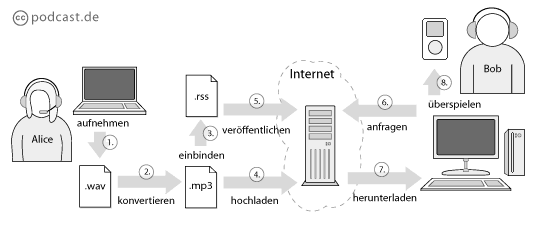
\includegraphics[width=10cm]{Bilder/podcast_prinzip_de.png}
\caption{Schematische Darstellung - Vom Producer zum Hörer \cite{FabioBacigalupo2004}}
\label{Podcastabruf}
\end{center}
\end{figure} 
\noindent \textit{Podcasting} ist das Produzieren von Video- oder Audioinhalten, die anschließend eine Verbreitung als Datei in einem \ac{RSS}-Feed finden. Bei Podcasts handelt es sich um eine Art Rundfunksendung, die zeitsouverän auf einem mobilen Gerät ohne Rundfunk- oder Datenempfang gehört oder gesehen werden kann. \\Seit 2004 weicht die digitale Bereitstellung von Informationen und Inhalten die bestehende Verbindung zwischen Inhalt und Medium vollends auf und ermöglicht einen selbstbestimmten und Medium-übergreifenden Konsum von Informationen und Inhalten. In der Konsequenz ist die ehemals unumstößliche Linearität der Medienlandschaft einer zeitlichen, räumlichen und inhaltlichen Flexibilisierung von Inhalten gewichen \cite[S. 19]{Daenzler2014}. \\
Heutzutage ist es ohne immensen technischen Aufwand und ohne umfassendes technisches Wissen möglich, an einem Computer mit Mikrofon und Internetanschluss einen Podcast zu erstellen. Die \textit{Abbildung \ref{Podcastabruf}} zeigt dies exemplarisch. Die Audio- oder Videodateien werden nach einer Konvertierung\footnote{Konvertierung bezeichnet in der Informatik die Überführung einer Datei von einem Dateiformat in ein anderes mittels einer Software. Wie hier .wav zu .mp3.} auf einen Webspace geladen und in die \ac{RSS}-Datei des Podcasts-Feeds eingebunden. Diese kann dann vom Hörer mit einem \textit{Podcasting-Client} (engl. Podcatcher) ausgelesen und abonniert werden. Der \textit{Podcatcher} lädt dann automatisch nach Erscheinen die neuen Podcast-Episoden auf das Endgerät des Hörers, der diese dann jederzeit konsumieren kann  (\textit{siehe Abbildung \ref{Podcastabruf}).}\\
\ac{RSS} ist ein auf \ac{XML} basierendes Format, welches entwickelt wurde, um Nachrichten und Web-Inhalte auszutauschen. \ac{XML} ist eine erweiterbare Auszeichnungssprache zur Darstellung hierarchisch strukturierter Daten im Format einer Textdatei und somit ohne großes Vorwissen nutzbar. Die \ac{RSS}-Datei enthält Metadaten (Metainformationen) des Podcasts, sowie der einzelnen Episoden. Diese Metadaten können grundlegende Informationen wie Titel, Autor, URL zum Titelbild, Episodentitel, kurze Zusammenfassung und den Link zur jeweiligen Episode enthalten. Aktuell gibt es starke Bestrebungen in Richtung des sogenannten Enhanced Podcasts. Dieser bietet darüber hinaus noch die Möglichkeit, Lesezeichen, erweiterte Textinformationen und Kapitel mit passenden Kapitelbildern für jede Podcast-Episode einzurichten. Für den Enhanced Podcast gibt es bisher keine einheitliche Spezifikation. Daher unterstützen verschiedene Medienplayer unterschiedliche Funktionen, was dem Konsumenten durchaus Schwierigkeiten bereiten kann. \ac{RSS} wird vom \ac{RSS} Advisory Board normiert und herausgegeben, dies ist für Podcast-Producer damit auch eine wichtige Quelle für die Weiterentwicklung des eigenen Podcasts \cite{RSSAB1999}.

\subsection{Audio-Podcast}
Wenn darüber gesprochen wird, einen Podcast zu konsumieren, dann ist damit meist der Audio Podcast gemeint. Die Entwicklung des Podcasts hat mit Audiobeiträgen begonnen und wurde viele Jahre von ihnen vorangetrieben, daher ist diese Art des Podcasts am verbreitetsten. Aber auch die einfache Art des Konsumierens ist ausschlaggebend. Audiodateien können ohne großen technischen Aufwand über Smartphones oder andere mobile Geräte wiedergegeben werden und erreichen damit schnell ein großes Publikum. An erster Stelle sind hier die täglichen Wege, die zurückgelegt werden müssen, zu nennen. Ob mit dem Auto, Nahverkehr, Fahrrad oder zu Fuß, Audio-Podcasts sind Begleiter, die Wissen liefern, ohne dabei von der eigentlichen Tätigkeit, der Fortbewegung, abzulenken. Dies macht es für viele attraktiv, sich auf dem morgendlichen Weg statt Musik einen Podcast zu einem für sie interessanten Thema anzuhören.\\
Der ausliefernde \ac{RSS}-Feed hatte eigentlich die Funktion der Nachrichtenverbreitung in Textform. Durch die Nutzung als Feed für Podcasts entstehen Definitionslücken, die dazu führen, dass es bisher keine genaue Spezifikation gibt, welche Art von Audiodatei ausgeliefert werden muss. Daher orientieren sich viele Producer an den Abspielformaten der großen Medienplayer, welche Codecs\footnote{Als Codec bezeichnet man einen Algorithmus, der Daten oder Signale digital kodiert und dekodiert.} dort nativ abspielbar sind. Die größte Verbreitung hat infolgedessen \ac{MP3} und \ac{AAC}. Da sich aber die Podcast-Community mit der Open-Source-Community maßgeblich überschneidet, sind auch exotischere Formate wie \ac{FLAC} oder \ac{Ogg Vorbis} zu finden.

\subsection{Videocast}
Der Videocast oder auch Video-Podcast\footnote{Teilweise auch Vodcast genannt.} ist eine Abwandlung des Audio-Podcasts, welche mit der weiteren technischen Entwicklung möglich wurde. Ab 2006 besaßen nach und nach immer mehr Computer, und später auch mobile Geräte, eine eingebaute Kamera, die es ermöglichte zusätzlich zum Audio auch das Video aufzuzeichnen. Die immer schnelleren Datenverbindungen ins Internet ermöglichten diese Weiterentwicklung des klassischen Podcasts. Die Videocast-Dateien wurden anfänglich über die eigene Webseite meist im Format der \ac{MPEG} zur Verfügung gestellt. Durch die große Marktmacht von Videoportalen wie YouTube\footnote{https://www.youtube.com (zuletzt zugegriffen 18.06.2018) \cite{YouTubeLLC}} oder Vimeo\footnote{https://vimeo.com (zuletzt zugegriffen 18.06.2018) \cite{Inc.}}, werden die meisten Videocasts inzwischen dort hochgeladen und durch den Anbieter in verschiedensten Formaten und Auflösungen zur Verfügung gestellt. Da die Anbieter meist eine Vielzahl von Formaten unterstützen, kann der Producer seiner Aufnahme- und Bearbeitungsumgebung individualisieren und braucht nicht mehr auf Kompatibilität zu achten.\\
Neben den zum Teil sehr professionellen Anbietern von Videocasts, wie der Bundeskanzlerin Angela Merkel \cite{Merkel2006} oder verschiedensten Firmen und Medienhäusern, die ihre Themen oder ihr Unternehmen bekannt machen wollen, gibt es auch viele Privatpersonen, die aus der intrinsischen Motivation Videocasts produzieren. 

\subsection{Sonderformen}
\frqq Das Abonnieren und Herunterladen von Podcasts ist für den Hörer kostenfrei.\flqq\,Diese Aussage lässt sich zwischenzeitlich nur noch eingeschränkt tätigen. Denn mit Plattformen wie Spotify\footnote{https://www.spotify.com (zuletzt zugegriffen 18.06.2018) \cite{SpotifyAB}}, Audible\footnote{https://www.audible.de (zuletzt zugegriffen 18.06.2018) \cite{AudibleGmbH}} oder Deezer\footnote{https://www.deezer.com (zuletzt zugegriffen 18.06.2018) \cite{DeezerGmbH}} gibt es inzwischen große Content-Plattformen, die nur kostenpflichtig zu nutzen sind. In der Podcast-Community wird der dort gelistete Content jedoch nicht als Podcast verstanden, da er dem Grundgedanken des freien und dezentralen Konsumieren von Medieninhalten widerspricht. Dennoch erreichen diese Plattformen durch ihre Marktmacht ein großes Publikum und prägen dadurch wiederum ihrerseits den Begriff ``Podcast`` in einer anderen Weise.\\
Neue Entwicklungen sind beispielsweise Videocasts, auf die der Nutzer Einfluss nehmen kann. Hier gibt es die Möglichkeit, Fragen in den Stream einzubauen, die der Nutzer beantworten muss, damit der Podcast weiter läuft. Je nachdem wie seine Antwort ausfällt, kann das Video unterschiedlich weitergehen. Dies zeigt die uBRAIN-Initiative in einem Beispielvideo\footnote{https://ubrain.info/digitale-bildung (zuletzt zugegriffen 20.06.2018) \cite{BNUG2016}}, welches als interaktives Video ein Showcase für weiteren Content sein soll.\\
Eine weitere Sonderform ist die Nutzung von Live-Streams für Podcast-Aufzeichnungen. Podcasts, welche bereits ein großes Publikum erreichen, stellen nicht nur, wie für Podcasts üblich, ihre Sendungen als \ac{RSS}-Feed zur Verfügung, sondern auch als Live-Stream. Hier wird die eigentliche Aufzeichnung zum Event und bietet den Konsumenten das Hören oder auch Sehen während der Aufzeichnung. Durch parallel stattfindende Chats wird der Hörer vom Konsumenten zum Beteiligten. Dies ist regelmäßig bei der Freakshow\footnote{https://freakshow.fm/live (zuletzt zugegriffen 22.06.2018) \cite{MPM2008}} zu beobachten.

\subsection{Notwendige Hardware}
Um heutzutage einen Podcast zu hören oder zu sehen, ist keine zusätzliche Hardware oder kein besonderes Equipment notwendig. Jedes handelsübliche Smartphone bietet bereits als Grundausstattung eine Podcast \ac{App} an oder sie ist kostenfrei in einem \ac{App}-Store der Plattform zu erhalten. Im Juni 2018 hat Google mit seiner neue Podcast-\ac{App} als letzter großer Marktteilnehmer nachgezogen und bietet nun eine eigene \ac{App} an \cite{Newton2018}. Podcast-\ac{App}s nehmen dem Nutzer das Handling mit \ac{RSS}-Feeds ab und zeigen beispielsweise in einer Listenansicht die Podcasts, welche der Nutzer hören oder abonnieren kann. Aber auch kostenpflichtige \ac{App}s sind nicht unüblich. Diese bieten dann zusätzliche Funktionen und Ansichten, die dem Konsumenten einen leichteren Zugang bieten oder sich besser individualisieren lassen.\\
Auch auf Desktop-PCs oder Macs gibt es entsprechende Programme. Da sich dort aber der Konsum anders verhält, ist die Auswahl bei weitem nicht so umfangreich. Der Konsum der Podcasts durch Browser ist hier der üblichere Weg. Eine zusätzliche Software ist daraus folgend für den Hörer selten nötig, ganz im Gegensatz zum Podcast-Producer. Dieser muss seinen Podcast für den Browser optimal aufbereiten, auf seiner Webseite präsentieren oder eines der großen Audio- und/oder Videoportale nutzen. 

\subsection{Plattformen}
Viele Plattformen bieten inzwischen umfangreiche Services und Angebote für Podcast Producer an. Besonders beliebt sind Plattformen wie iTunes\footnote{https://www.apple.com/de/itunes (zuletzt zugegriffen 18.06.2018) \cite{Apple2001}}, die vom Producer nur den Link zum Podcast \ac{RSS}-Feed benötigen um den Podcast im Verzeichnis allen Hörern anzubieten. \\
In Konkurrenz zu der Podcast-Community steht inzwischen der öffentlich-rechtliche Rundfunk mit seinen Mediatheken. Viele seiner Rundfunk- und Fernsehsendungen gibt es nicht nur dort, sondern auch mittels eines \ac{RSS}-Feeds als Podcast. Auch in den großen Verzeichnissen werden diese Inhalte gelistet. Diese Konkurrenz von umfangreichen und qualitativ gut produzierten Inhalten nötigt jedoch auch Producer freier Podcasts zu einer hohen Mindestqualität, damit die Nutzer erreicht werden können. Für die Konsumenten kann dieses größere Angebot und die gesteigerte Qualität von Vorteil sein.\\
Als eine der größten Plattformen ist hier noch YouTube zu nennen. YouTube bietet inzwischen im großen Umfang Podcasts, besonders für Lernende, an. Aber YouTube agiert nicht nur als Plattform für Inhalte, sondern unterstützt die Producer durch die sogenannten YouTube Spaces\footnote{https://www.youtube.com/intl/de/yt/space/ (zuletzt zugegriffen 19.06.2018) \cite{YouTubeLLC2005}} direkt bei der Produktion ihres Contents. Hier werden den Producern professionelles Equipment, Räume und Coaching zur Verfügung gestellt. Zusätzlich haben bekannte YouTuber nicht unerhebliche Werbeeinnahmen von zum Teil mehreren Hunderttausend Euro im Jahr  \cite{Statista2017}. In der Liste der Podcaster mit den höchsten Werbeeinnahmen verbirgt sich jedoch kein einziger mit Bildungsthemen. 

\subsection{Fehlende Verweise und Quellen}
Podcasts haben allgemein das Problem, dass Verweise und Links zu Quellen dem Konsumenten schwer zu vermitteln sind. Bei Audio-Podcasts gibt es zwar über die so genannten Shownotes\footnote{Häufig werden Podcasts zusammen mit ergänzenden Sendungsnotizen zur aktuellen Episode veröffentlicht. Diese sogenannten Shownotes enthalten meist neben einem beschreibenden Text auch Bilder und Links zu den besprochenen Themen.}, also den zusätzlichen Textfeldern der \ac{RSS}-Datei, die Möglichkeit, Links und Quelleninformationen mitzugeben. Jedoch werden Audio-Podcasts vielfach unterwegs auf dem Smartphone konsumiert, während das Display abgeschaltet ist.\\ Aber auch bei Videocasts sind Quellenangaben häufig nur in den meist nicht vollständig eingeblendeten Begleittexten zu finden. Ein Einbetten in das Video selbst ist zwar möglich, wird aber vornehmlich aus ästhetischen Gründen nicht gemacht. Zusätzlich führt ein Klicken auf einen weiterführenden Link den Konsumenten direkt vom Podcast weg, was in der Regel nicht gewünscht ist.\\
Dies führt zu dem Phänomen, dass Wissen vermittelt wird, aber der Konsument Fakten schwer nachvollziehen kann. Vertrauen in den Producer des Podcasts und dessen Integrität ist hier die Voraussetzung. Dies muss sich auch der Producer klar machen, denn ein Weitergeben von falschen Informationen oder Fehlinterpretationen kann für seine Konsumenten zum Problem werden. Besonders Lernende im schulischen oder universitären Kontext sind darauf angewiesen besonders, gut recherchierte Informationen und nachprüfbare Quellen als zusätzliche Information angeboten zu bekommen.

\section{Lernen mit Podcasts}
Die Vokabelkassetten, auf denen Wörter einer Fremdsprache vorgelesen und übersetzt werden, sind heute eher unüblich. Hier hat sich die Entwicklung des Podcasts niedergeschlagen, welcher im schulischen oder universitären Umfeld gern Educast genannt wird. Sogennante Educasts werden als pädagogisch motivierte Podcasts zur Wissensvermittlung und zum Lernen produziert\\ \cite{MandySchiefner2008}. \\ 
Zusätzlich gibt es nicht nur ein natives fremdsprachiges Angebot von Podcastern aus aller Welt, sondern es gibt speziell für das Erlernen einer Sprache Podcasts. Diese machen in ihren Episoden das Lernen von Fremdwörtern und das Verbessern rezeptiver Fertigkeiten fast zur Nebensache und vermitteln auch kulturelles oder gesellschaftliches Wissen. So bietet die BBC bereits seit 2010 verschiedenen Podcasts zum Lernen und Verstehen der englischen Sprache an, wie zum Beispiel ``The English We Speak`` . In diesem Podcast werden Wörter oder Phrasen besprochen, die helfen, besser English zu sprechen und zu verstehen \cite{BBCRadio2010}. Aber auch in Deutschland haben Nachrichtenportale den Mehrwert erkannt, Nachrichten durch Podcasts an Menschen zu vermitteln, die eine Sprache nicht gut sprechen oder diese erlernen wollen. Die Deutsche Welle bietet nicht nur fremdsprachiges Material an, sondern auch Nachrichten in Deutsch, die besonders langsam und betont gesprochen werden \cite{Welle2018}.

\subsection{Mehrwert durch Podcasts}
Um einen Mehrwert für Lernende durch Podcasts zu erzeugen, braucht es zusätzliche Arbeit durch den Producer. Einen Lehrtext zu lesen oder ihn als Podcast vorgetragen zu bekommen, bringt dem Lernenden keinen zeitlichen Mehrwert. Hier mag nur derjenige Vorteile aus der Darreichungsform ziehen, der einer bessere auditive Wahrnehmung besitzt und hierdurch mehr des zu lernenden Stoffes aufnehmen kann.\\
Hingegen ist Reisen oft eine Zeit, in der Menschen sich weniger kognitiv betätigen. Dies deutet darauf hin, dass Podcasts eine wichtige Bedarfslücke schließen können. Es wird dem Lernenden erlaubt, die Lernaktivitäten fortzusetzen, an Orten wo dies normalerweise nicht möglich ist. Bei Reisen geht aber ein wichtiger Aspekt des Lernens verloren. Durch den beengten Raum, oder die eigene Bewegung während des Reisens, ist es nicht möglich eigene Notizen zum erlernten Stoff anzufertigen. Ein Aspekt, der gerade im lernenden Kontext wichtig ist.\\
Grundsätzlich erfordert das Hören von Podcasts aber eine hohe Aufmerksamkeit. Multi-Tasking ist scheinbar nicht möglich \cite{Evans2008}.

\subsubsection{Nutzung durch Lernende}
Lee und Chan zeigten 2007, dass Studierende sowohl in den traditionellen als auch in Fernkursen die Audio Podcasts meist auf einem Desktop-Computer zu Hause oder in ihren Wohnheimen hören und nicht unterwegs auf einem mobilen Gerät. Darüber hinaus sagten die meisten Studierende, dass sie Podcasts hörten, ohne sich mit anderen Aktivitäten zu beschäftigen. Diese Ergebnisse deuten darauf hin, dass eher Eindrücke oder Überzeugungen als empirische Beweise als Grundlage für die Argumentation verwendet werden, dass Podcasting den Lernenden eine Multitasking-Möglichkeit bietet und ein hohes Maß an Lifestyle-Integration fördert \cite{LeeChan2007}.\\
Dies legt die Vermutung nahe, dass eine mobile Weiterbildung durch Podcasts durchaus möglich ist, für Schüler/Schülerinnen und Studierende aber eine eher untergeordnete Rolle spielt. Erworbenes Wissen wird erwartbar abgefragt, was es notwendig macht, die vermittelten Inhalte möglichst vollumfänglich aufzunehmen. Dafür sind eigene Notizen notwendig, die mangels der Situation nicht unterwegs in gleicher Qualität und Quantität entstehen können.\\
Wenn es keine parallele Aktivität gibt und eine mobile Nutzung zum Lernen eine untergeordnete Rolle spielt, ist an dieser Stelle der Videocast zu betrachten. Dieser wird durch sein Format häufig am Computer konsumiert. Das notwendige Verfolgen eines Videos und der deutlich höhere Datenverbrauch bei einer mobilen Ansicht sind hier als Gründe zu nennen.\\
Nehmen wir uns beispielhaft die zwei bekanntesten Erklärpodcasts für Mathematik Themen in Deutschland. Die beiden Videocasts ``TheSimpleMaths``\footnote{https://www.youtube.com/TheSimpleMaths (zuletzt zugegriffen 19.06.2018) \cite{YouTubeMath_2011}} und ``Mathe by Daniel Jung``\footnote{https://www.youtube.com/user/beckuplearning/featured (zuletzt zugegriffen 19.06.2018) \cite{YouTubeJung_2011}} präsentieren in kurzen 3-9-Minuten-Videos ein einzelnes Thema der Mathematik. Hier wird die Berechnung einer Nullstelle erklärt oder über Quadratische Funktionen gesprochen. Auf den ersten Blick sind das nicht unbedingt Themen, mit denen Jugendliche, und damit die Zielgruppe, auf lange Sicht gebunden werden können. Anhand der Nutzerzahlen zeigt sich aber klar ein anderes Bild. So wurden einzelne Videos bis zu 1,6 Millionen Mal (TheSimpleMaths), bzw. 880.000 mal (Mathe by Daniel Jung) angesehen. Alle Videos der Kanäle summieren sich zu  93 Millionen bzw. 128 Millionen Views (Stand: Juni 2018) \cite{YouTubeMath_2011} \& \cite{YouTubeJung_2011}. Dies zeigt, was für eine hohe Nachfrage selbst schwer zugängliche Themen haben können, wenn sie in kurzer und prägnanter Weise als Podcast zur Verfügung gestellt werden.\\
Podcasts können für Lernende aber auch einen zusätzliche Nutzen haben, wenn sie ihn selber produzieren müssen. Neben der digitalen Weiterbildung, weil das Setting und die Technik der Podcast-Produktion erlernt werden muss, wird das eigentliche Wissen, welches die Lernenden für den Podcast aufbereiten, verfestigt. Somit fördern Educasts ein konstruktivistisches Lernen. Wissen wird nicht vorgegeben und gelernt, sondern muss selbst erschlossen, verarbeitet, strukturiert und transferiert werden, um in die Konstruktion eigener kognitiver Schemata zu münden \cite[S. 260]{Zorn2013}. 

\subsection{Nutzung für Lehrkräfte}
Lehrkräfte können Podcasts zur Erweiterung ihres Unterrichts nutzen. So können Screencasts\footnote{Ein Screencast ist eine Video-Aufzeichnung, die Inhalte am Computer-Bildschirm wiedergibt und ggf. mit Audio-Kommentaren beschreibt.} aufgezeichnet werden, also Mitschnitte von Unterrichtsstunden oder Vorlesungen. Doch dieses nebenbei produzierte Lehrmaterial, das in Form von Podcasts in den meisten Fällen bei einer Vorlesung aufgezeichnet wird, ist dann nicht mediendidaktisch aufbereitet, sondern eine mediale Abbildung einer Universitätsvorlesung, die auch nach vorlesungsdidaktischen Aspekten geplant wurde. Unterrichtsmedien liegen aber andere didaktische Konzepte zugrunde als einer Präsenzveranstaltung. Somit ist eine aufgezeichnete Präsenzveranstaltung noch kein gutes Unterrichtsmedium \cite[S. 21]{MandySchiefner2008}.\\ Hochsam stellt die Sinnhaftigkeit von Aufzeichnungen ganzer Vorlesungen grundsätzlich in Frage, solange keine spezielle Didaktik für die Aufbereitung des Materials genutzt werde. Hier kann, laut seiner Schlussfolgerung, nur die Nutzung von Enhanced Podcasts helfen. Kapitelmarken und Suchfunktionen könnten seine Kritik relativieren \cite[S. 47]{JuergenHochsam2008}.\\
Dennoch haben die Lernenden die Möglichkeit, bei einem für sie schwierigen Thema, Inhalte solange sanktionsfrei immer wieder zu konsumieren, bis sie sich sicher fühlen. Wenn der Unterricht eine mediale Komponente besitzen soll, kann hier die Aufgabe darin bestehen, Gelerntes als Podcast aufzubereiten und für die Mitlernenden bereitzustellen.\\
Hier ist aber wichtig zu beachten, dass bei Minderjährigen die Verantwortlichkeit für die Inhalte im Podcast beim Lehrenden bzw. bei der Schulleitung liegt. Hier ist den Betroffenen die Brisanz der Nutzung von urheberrechtlich geschützten Inhalten deutlich zu machen. Daneben ist es wichtig, bei der Verwendung von personenbezogenen Daten wie Fotos und Namen von Minderjährigen die Erlaubnis der Eltern einzuholen \cite[S. 262]{Zorn2013}.\\
Auf Plattformen für Lehrmaterial wie Lehrer-Online\footnote{https://www.lehrer-online.de (zuletzt zugegriffen 17.06.2018) \cite{EduversumGmbH1999}} gibt es bereits seit einigen Jahren Anleitungen zum multimedialen Lernen oder auch ganze Unterrichtstunden als fertiges Konzept. Damit können Lehrkräfte, die bisher keinen Einstieg ins Podcasting gefunden haben, eine mögliche Nutzung für ihren Unterricht ausloten, denn das Nutzen von solchen Methoden fördert die Medienkompetenz der Lernenden, die wiederum eine Schlüsselkompetenz für die politische Urteils- und Handlungsfähigkeit ist. 

\subsubsection{Nutzung zur Weiterbildung}
Der Konsum von Podcasts und dessen Nutzung zur Weiterbildung ist nicht nur von der Situation abhängig, sondern auch von der Materie. Auch wenn es mit dem PriMaPodcast\footnote{Mathematische Audio-Podcasts in der Primarstufe} eine Idee der Umsetzung von mathematischen Inhalten auf einer ausschließlich sprachliche Ebene gibt, sind doch gerade Formeln und die Wissensweitergabe darüber besonders gut in Videocasts vermittelbar. Dies schließt eine Nutzung komplexer Themen in Audio-Podcasts jedoch nicht aus. Bei der Nutzung muss das Thema jedoch gut vorbereitet sein und sollte nicht zu kurz, sondern möglichst ausführlich abgehandelt werden. Dies zeigt sich sehr gut an einem der Podcast-Pioniere in Deutschland. Tim Pritlove stellt mit seinem Chaosradio Express\footnote{https://cre.fm (zuletzt zugegriffen 23.06.2018) \cite{TPPM2005}} bereits seit 2005 komplexe Themen umfassend und möglichst abschließend als Audio-Podcast der Allgemeinheit zur Verfügung.\\
Weiterbildung funktioniert aber auch besonders gut ortsgebunden, wenn zusätzliches Wissen als Audio-Podcast beispielsweise im Rahmen eines Nationalparkbesuchs zur Verfügung gestellt wird. Dies war bereits Thema der Forschung.\\
Die Untersuchung von Kang und Gretzel zeigt, dass die menschliche Stimme, auch wenn sie über reine Audio-Medien kommuniziert wird, einen positiven sozialen Rahmen für eine nachhaltige Entwicklung schafft und das touristische Erleben und die Verantwortung beeinflusst. Daher hat diese Studie den Nutzen von Podcast-Touren als Informationsmedium identifiziert. Die wahrgenommene soziale Präsenz wird erhöht, was wiederum zu einer Verbesserung der touristischen Erfahrungen und der Umweltverantwortung bei dem Besuch des Nationalparks führt \cite{Kang2012}.

\section{Ausblick}
Insgesamt gibt es gerade im schulischen und universitären Kontext das Problem, Wissen in optimaler Form mithilfe von Podcasts zu vermitteln. Einem/Einer Lernenden ist ein 90-minütiger Podcast keine Hilfe, wenn er eine bestimmte Frage zum Thema beantwortet haben will und der Inhalt nicht durchsuchbar ist. Wenn dann noch die unattraktive Form des Screencasts genutzt wurde, kann die intensive Nutzung und positive Einstellung der Lernenden gefährdet werden.\\
Hier sind also in erster Linie immer der Zweck und der Nutzen zu betrachten, bevor das Mittel der Lernmethode gewählt wird. So wird es für jede Art des Podcasts eine Zielgruppe und eine Anwendung geben. Die Anwendung der falschen Methode kann aber nicht nur durch ausbleibenden Lernerfolg gekennzeichnet sein, sondern schlimmstenfalls die gegenteilige Wirkung entfalten. Hier sollte also weiterführend geforscht werden, welche der vielen Podcast-Methoden, die zwischenzeitlich entstanden sind, für bestimmte Aspekte des Lernens von Vorteil und welche zu meiden sind. Das Ende des Podcast-Spektrums ist zwischenzeitlich noch nicht erreicht, wie zwei Beispiele zeigen, die sich in der Entwicklung befinden.\\
Mit dem neuen Projekt von James Ryan, Doktorand an der University of California, ist es möglich, dass sich die Podcast-Landschaft wieder erweitert. In dieser neuen Variante des Podcasts spricht nicht nur eine KI den Text des Podcasts, sondern entwickelt ihn selbständig von wenigen Grundfaktoren ausgehend auch inhaltlich weiter \cite{JamesRyan2018}.\\
Auch die Möglichkeit der interaktiven Videocasts, wie ihn uBRAIN\footnote{https://ubrain.info (zuletzt zugegriffen 20.06.2018) \cite{BNUG2016}} beispielhaft vorstellt, muss genauer betrachtet werden. Welchen Einfluss hat ein Videocast, wenn der Nutzer nicht mehr nur Konsument eines redaktionellen Podcasts ist, sondern durch aktives Einbinden in das Thema proaktiv wird. Der Videocast fragt nicht nur vorhandenes Wissen ab, sondern passt sich entsprechend der Antworten im weiteren Verlauf dem Wissensstand des/der Lernenden an. Dies kann im schulischen und universitären Kontext möglicherweise sinnvoll für das Lernen vor Prüfungen genutzt werden, da es sich an das Leistungsniveau des Lernenden anpasst und somit nicht die Gefahr besteht, einzelne abzuhängen.
 
%--- Für Quellen ist das Programm JabRef nötig ---
\renewcommand{\bibname}{Quellen}
\bibliography{Literatur}
\addcontentsline{toc}{chapter}{Quellen}
\thispagestyle{fancy}

\addchap{Abkürzungsverzeichnis}
\label{sec:abkuerzungsverzeichnis}
\thispagestyle{fancy}

\begin{acronym}[OOOOOOOO]
	\acro{AAC}{Advanced Audio Coding}
	\acro{App}{Application (Anwendungsprogramm)}
	\acro{FLAC}{Free Lossless Audio Codec}
	\acro{MP3}{MPEG Layer 3}
	\acro{MPEG}{Moving Picture Experts Group}
	\acro{NDR}{Norddeutscher Rundfunk}
	\acro{Ogg Vorbis}{Ogg Vorbis}
	\acro{RSS}{Rich Site Summary (später Really Simple Syndication)}
	\acro{VLog}{Video-Blog}
	\acro{XML}{Extensible Markup Language}

\end{acronym}

\end{document}